\section{Einleitung}

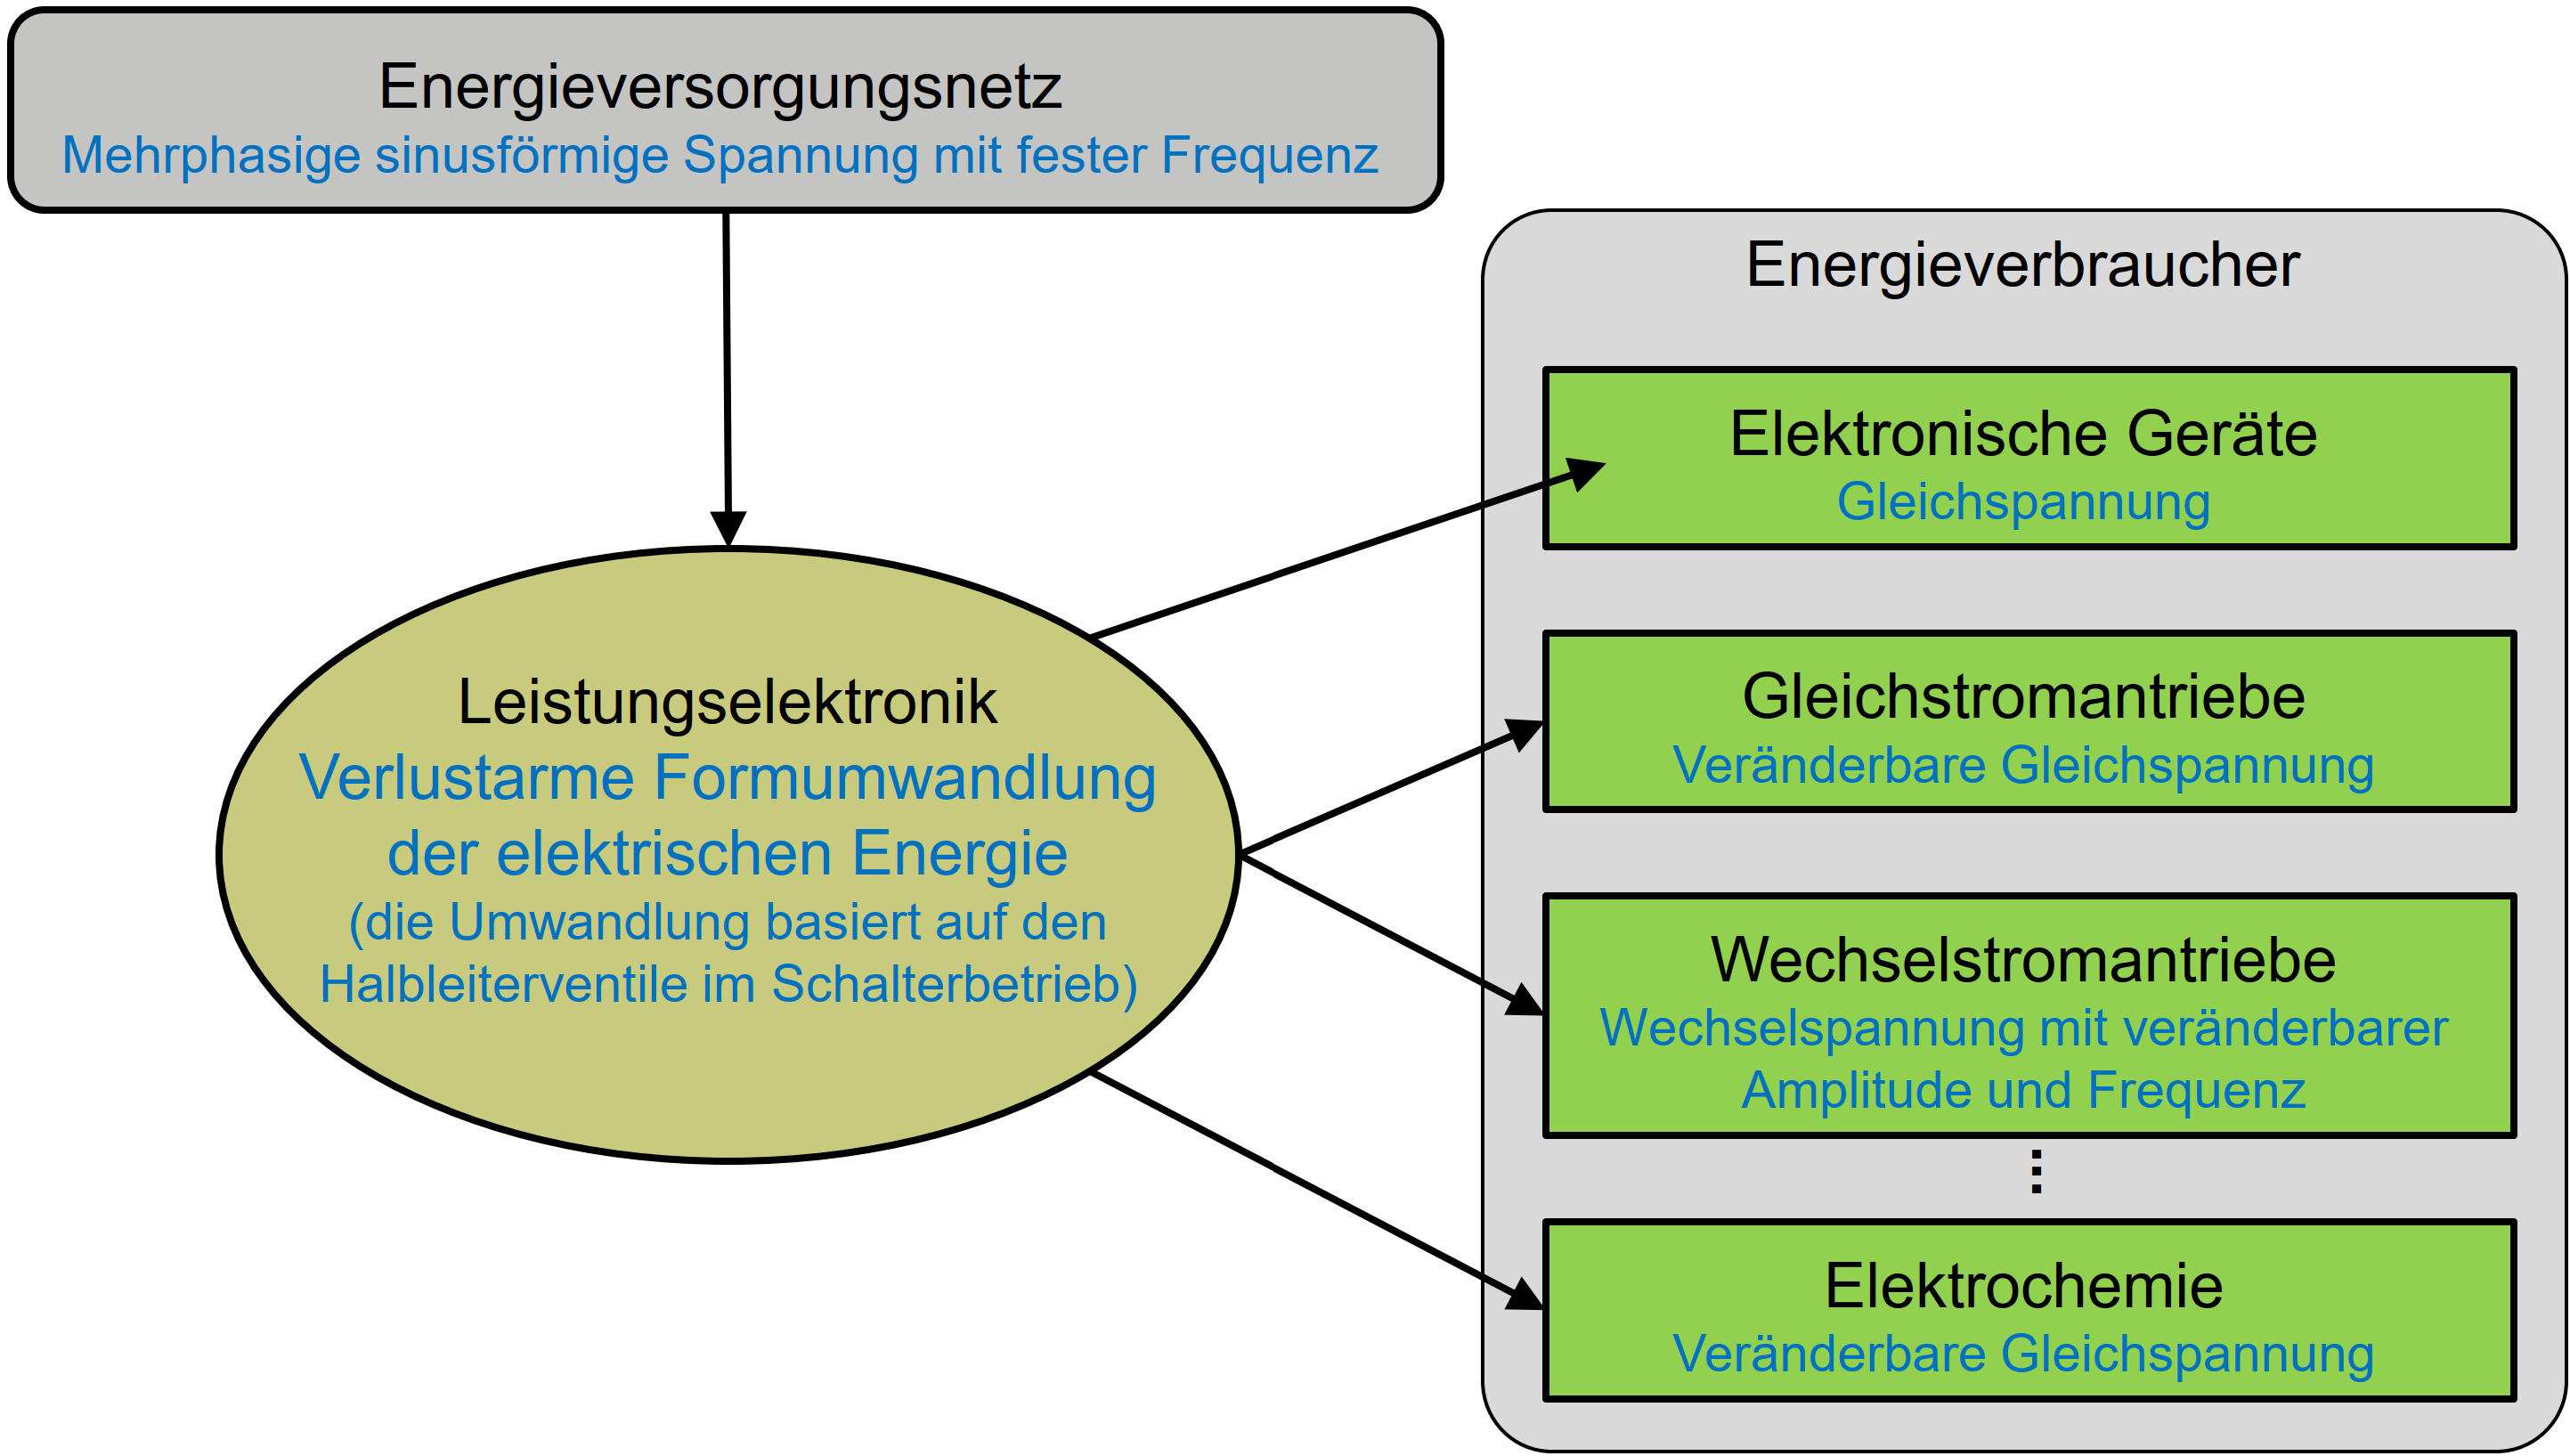
\includegraphics[width=\columnwidth]{images/Bild0.png}

\subsection{Definition des Gebiets der Leistungselektronik}
Schalten, Steuern und Umformen elektrischer Energie mit elektronischen Mitteln

\subsection{Grundfunktionen der Leistungselektronik}
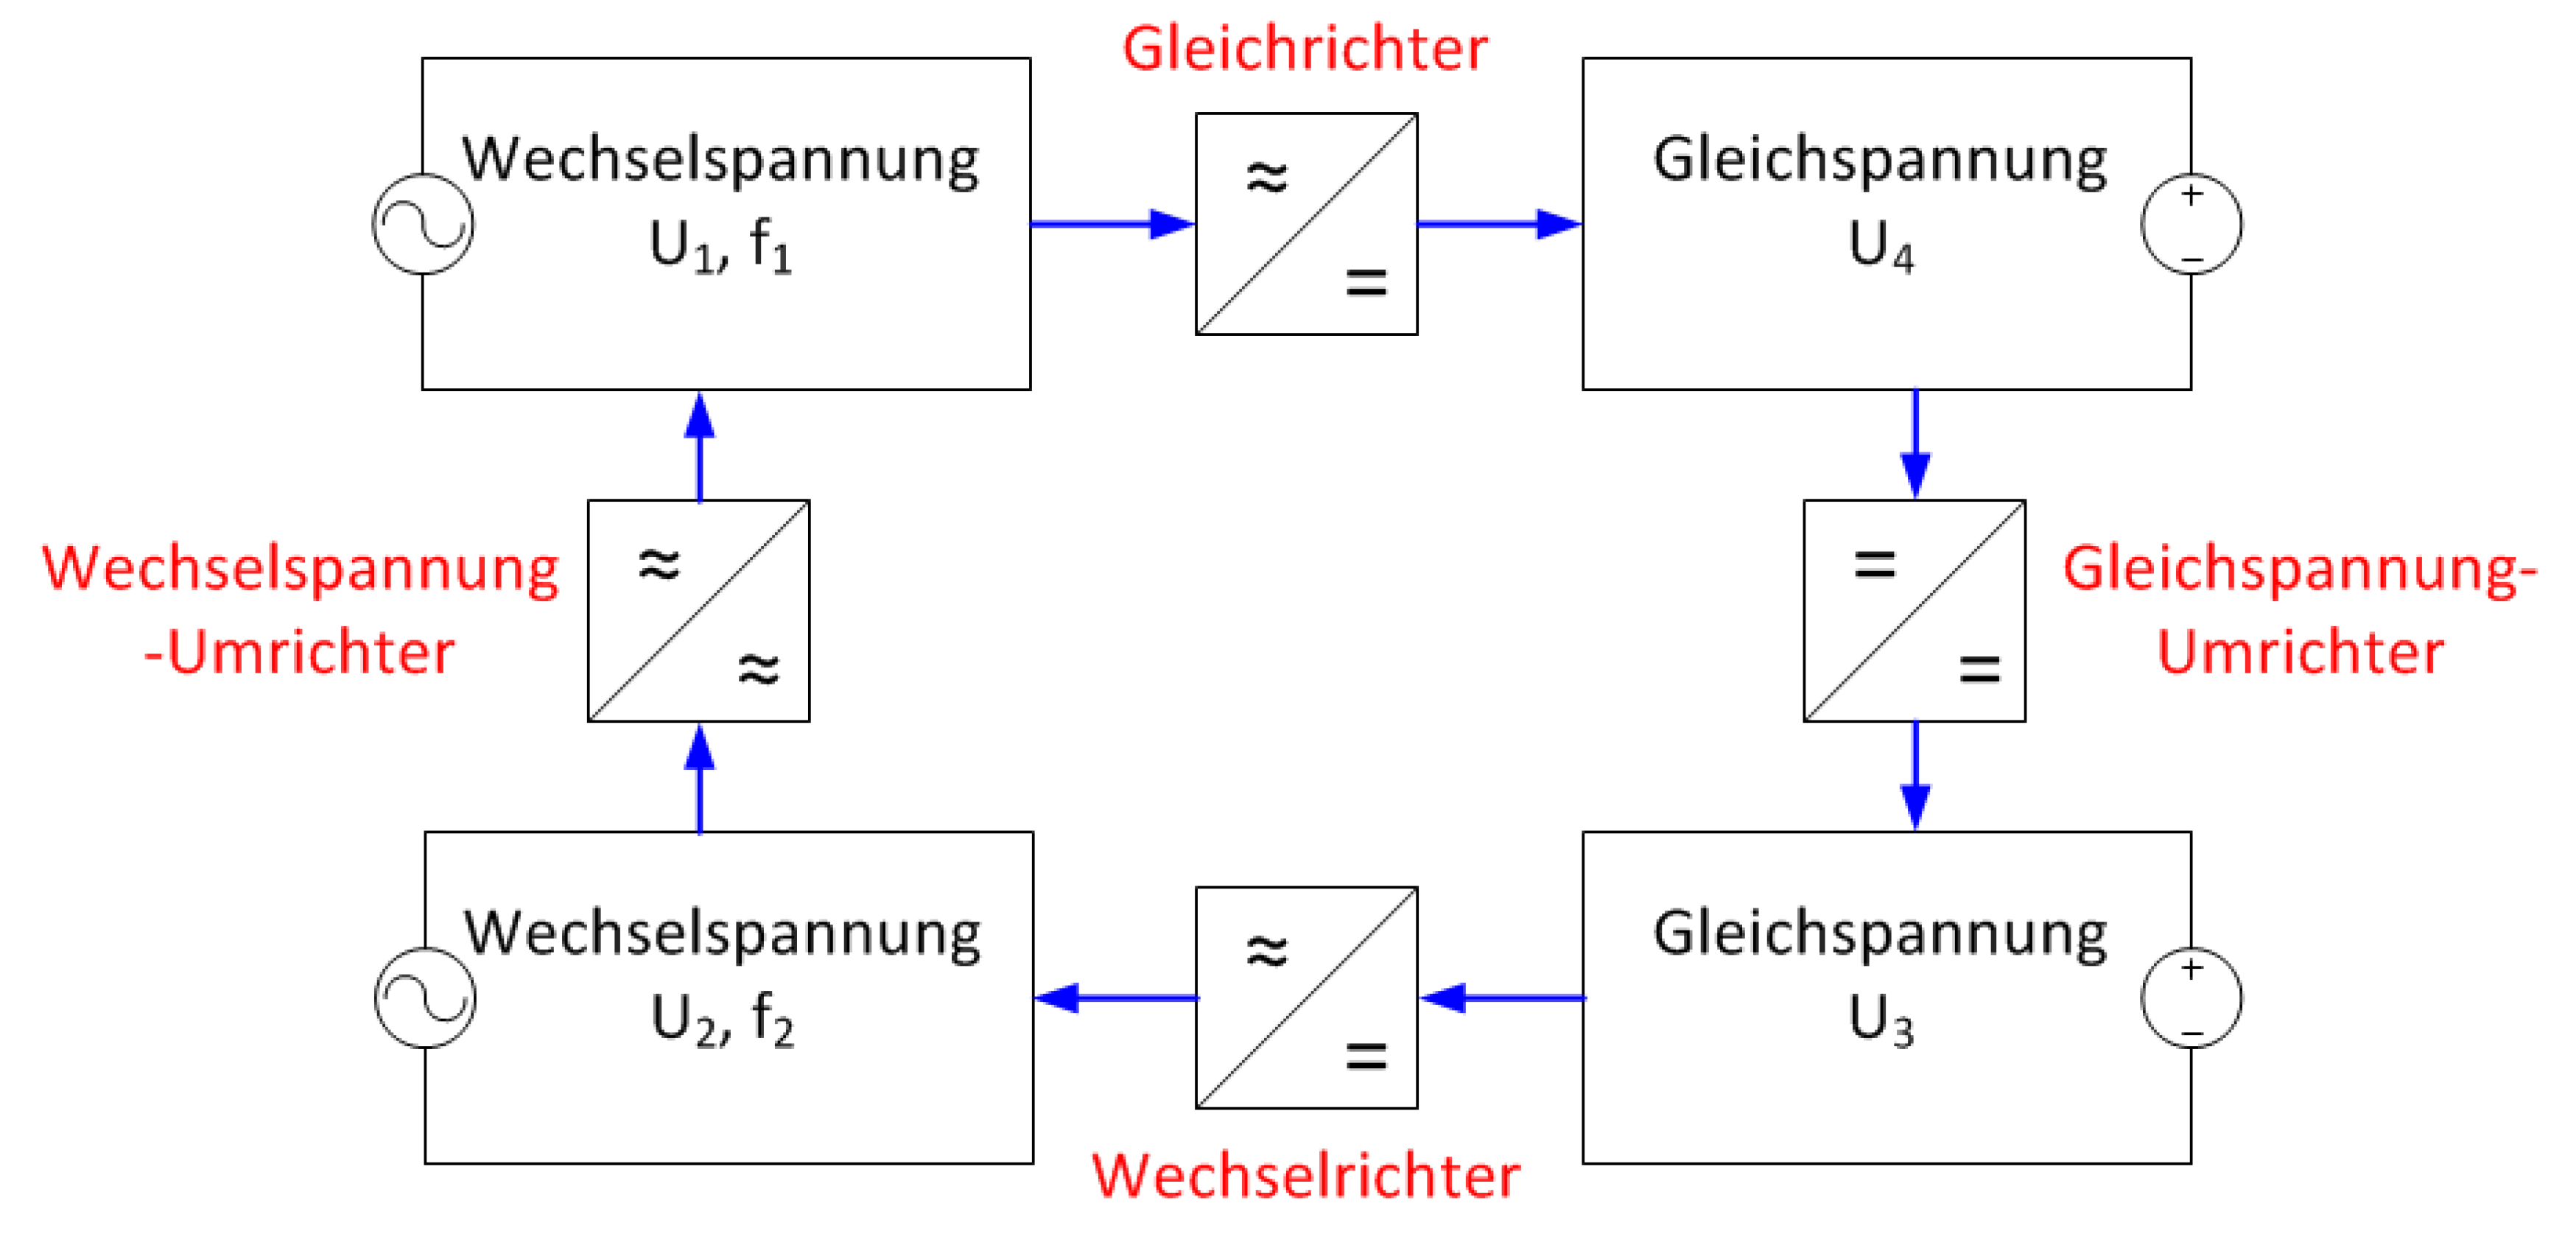
\includegraphics[width=\columnwidth]{images/Bild1.png}

\subsection{Halbleiterphysik}

\begin{itemize}
    \item \textbf{Metallische Leiter:} Der Stromtransport wurde durch Elektronen erzeugt.\\
    Der spezifische Widerstand des Kupfers bei $0^\circ C$:  $\rho = 1.56 \cdot 10^{-8} \, \Omega \text{m}$.
    \item \textbf{Isolatoren:} der Stromtransport wurde durch Ionen erzeugt.\\
    Der spezifische Widerstand des Quarzes bei $0^\circ C$: $\rho = 10^{14} \, \Omega \text{m}$.
    \item \textbf{Halbleiter:} die Leitfähigkeit liegt irgendwo zwischen Metallen und Isolatoren.\\
    Der spezifische Widerstand des Siliziums bei $0^\circ C$: $\rho = 10^4 \, \Omega \text{m}$.\\
    Die wichtigsten Halbleiter: Si, Ge, CuO$_2$, und GaAs.
    \item \textbf{Dotierte Halbleiter:} die reine Halbleiterwerkstoffe sind nicht so interessant.\\
    Jedoch kann man durch kontrollierte Verunreinigung (Dotieren) der reinen Halbleiterwerkstoffe die Leitfähigkeit 
    wesentlich ändern (um $10^{14}$).
\end{itemize}
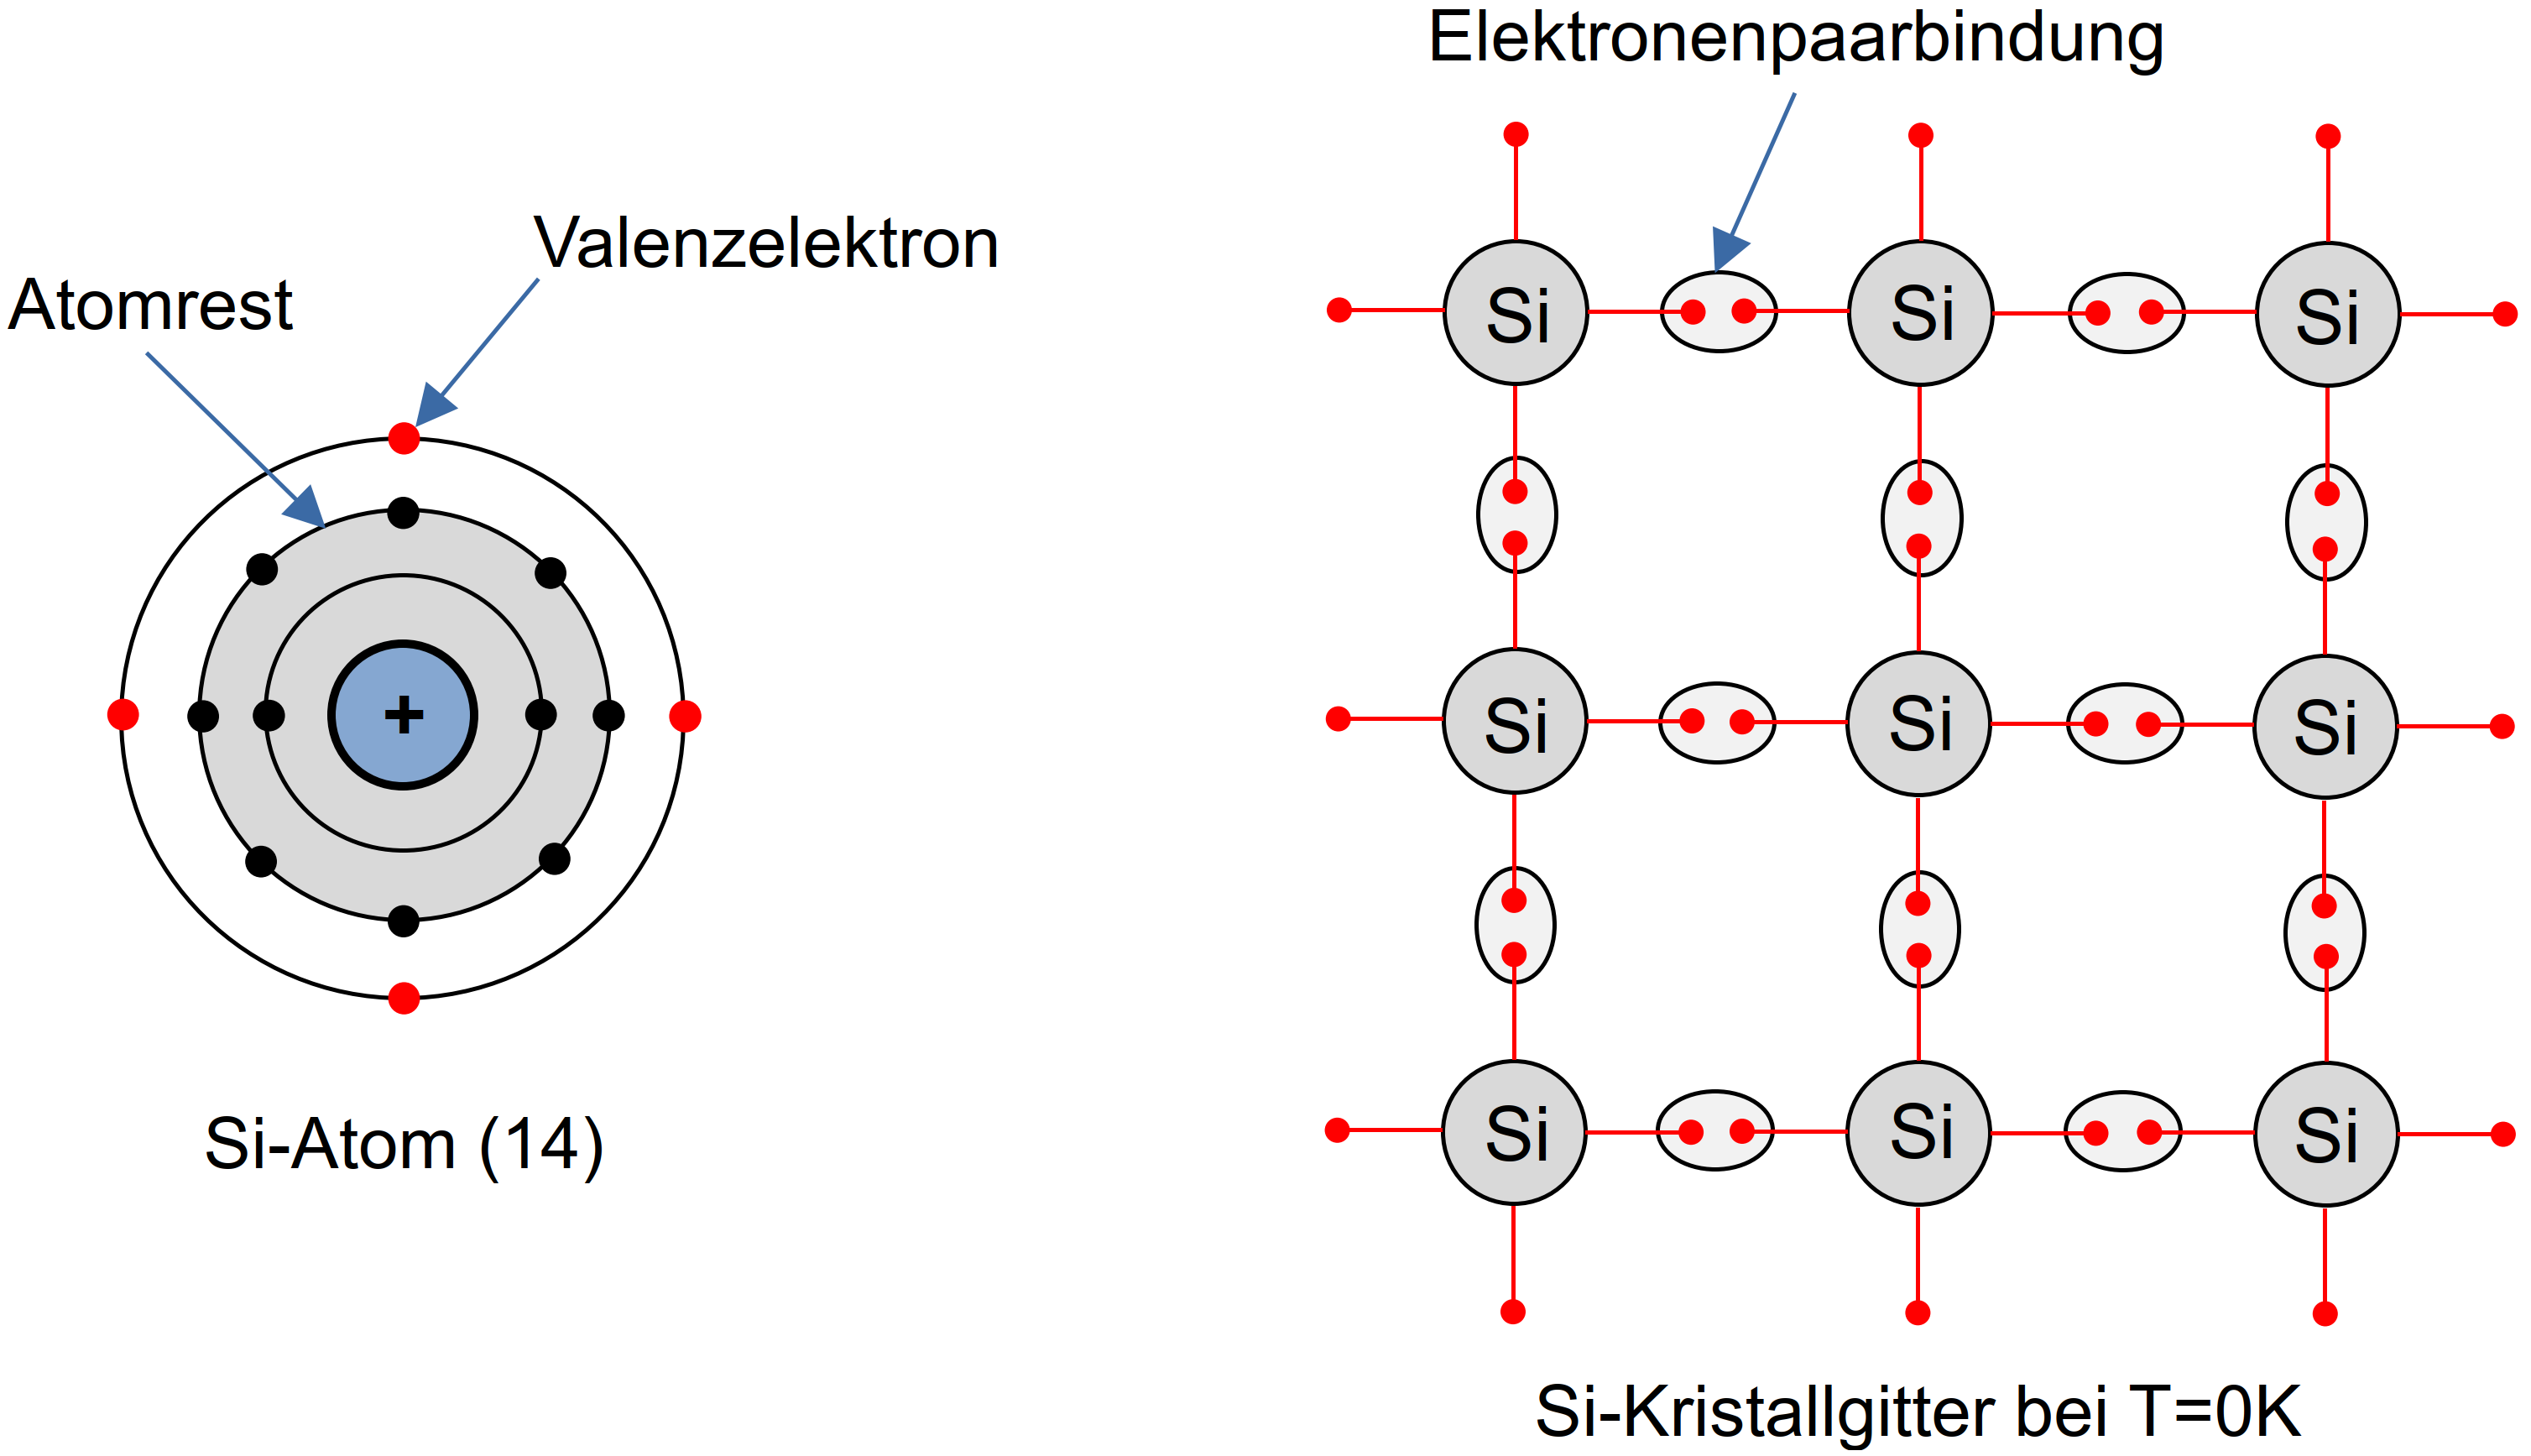
\includegraphics[width=\columnwidth]{images/Bild2.png}

\columnbreak
\subsubsection{Eigenleitung}
Durch die thermische Bewegung der Atomen um ihre Ruhelage im Kristallgitter ist es möglich 
einige \textbf{Elektronbindungen} aufzubrechen.\\ 
Auf diese weise ein \textbf{gelöstes Elektron} bewegt sich im Kristallgitter 
frei und hinterlässt eine positivgeladene \textbf{Lücke im Kristallgitter} (so genannte Loch oder Defektelektron).
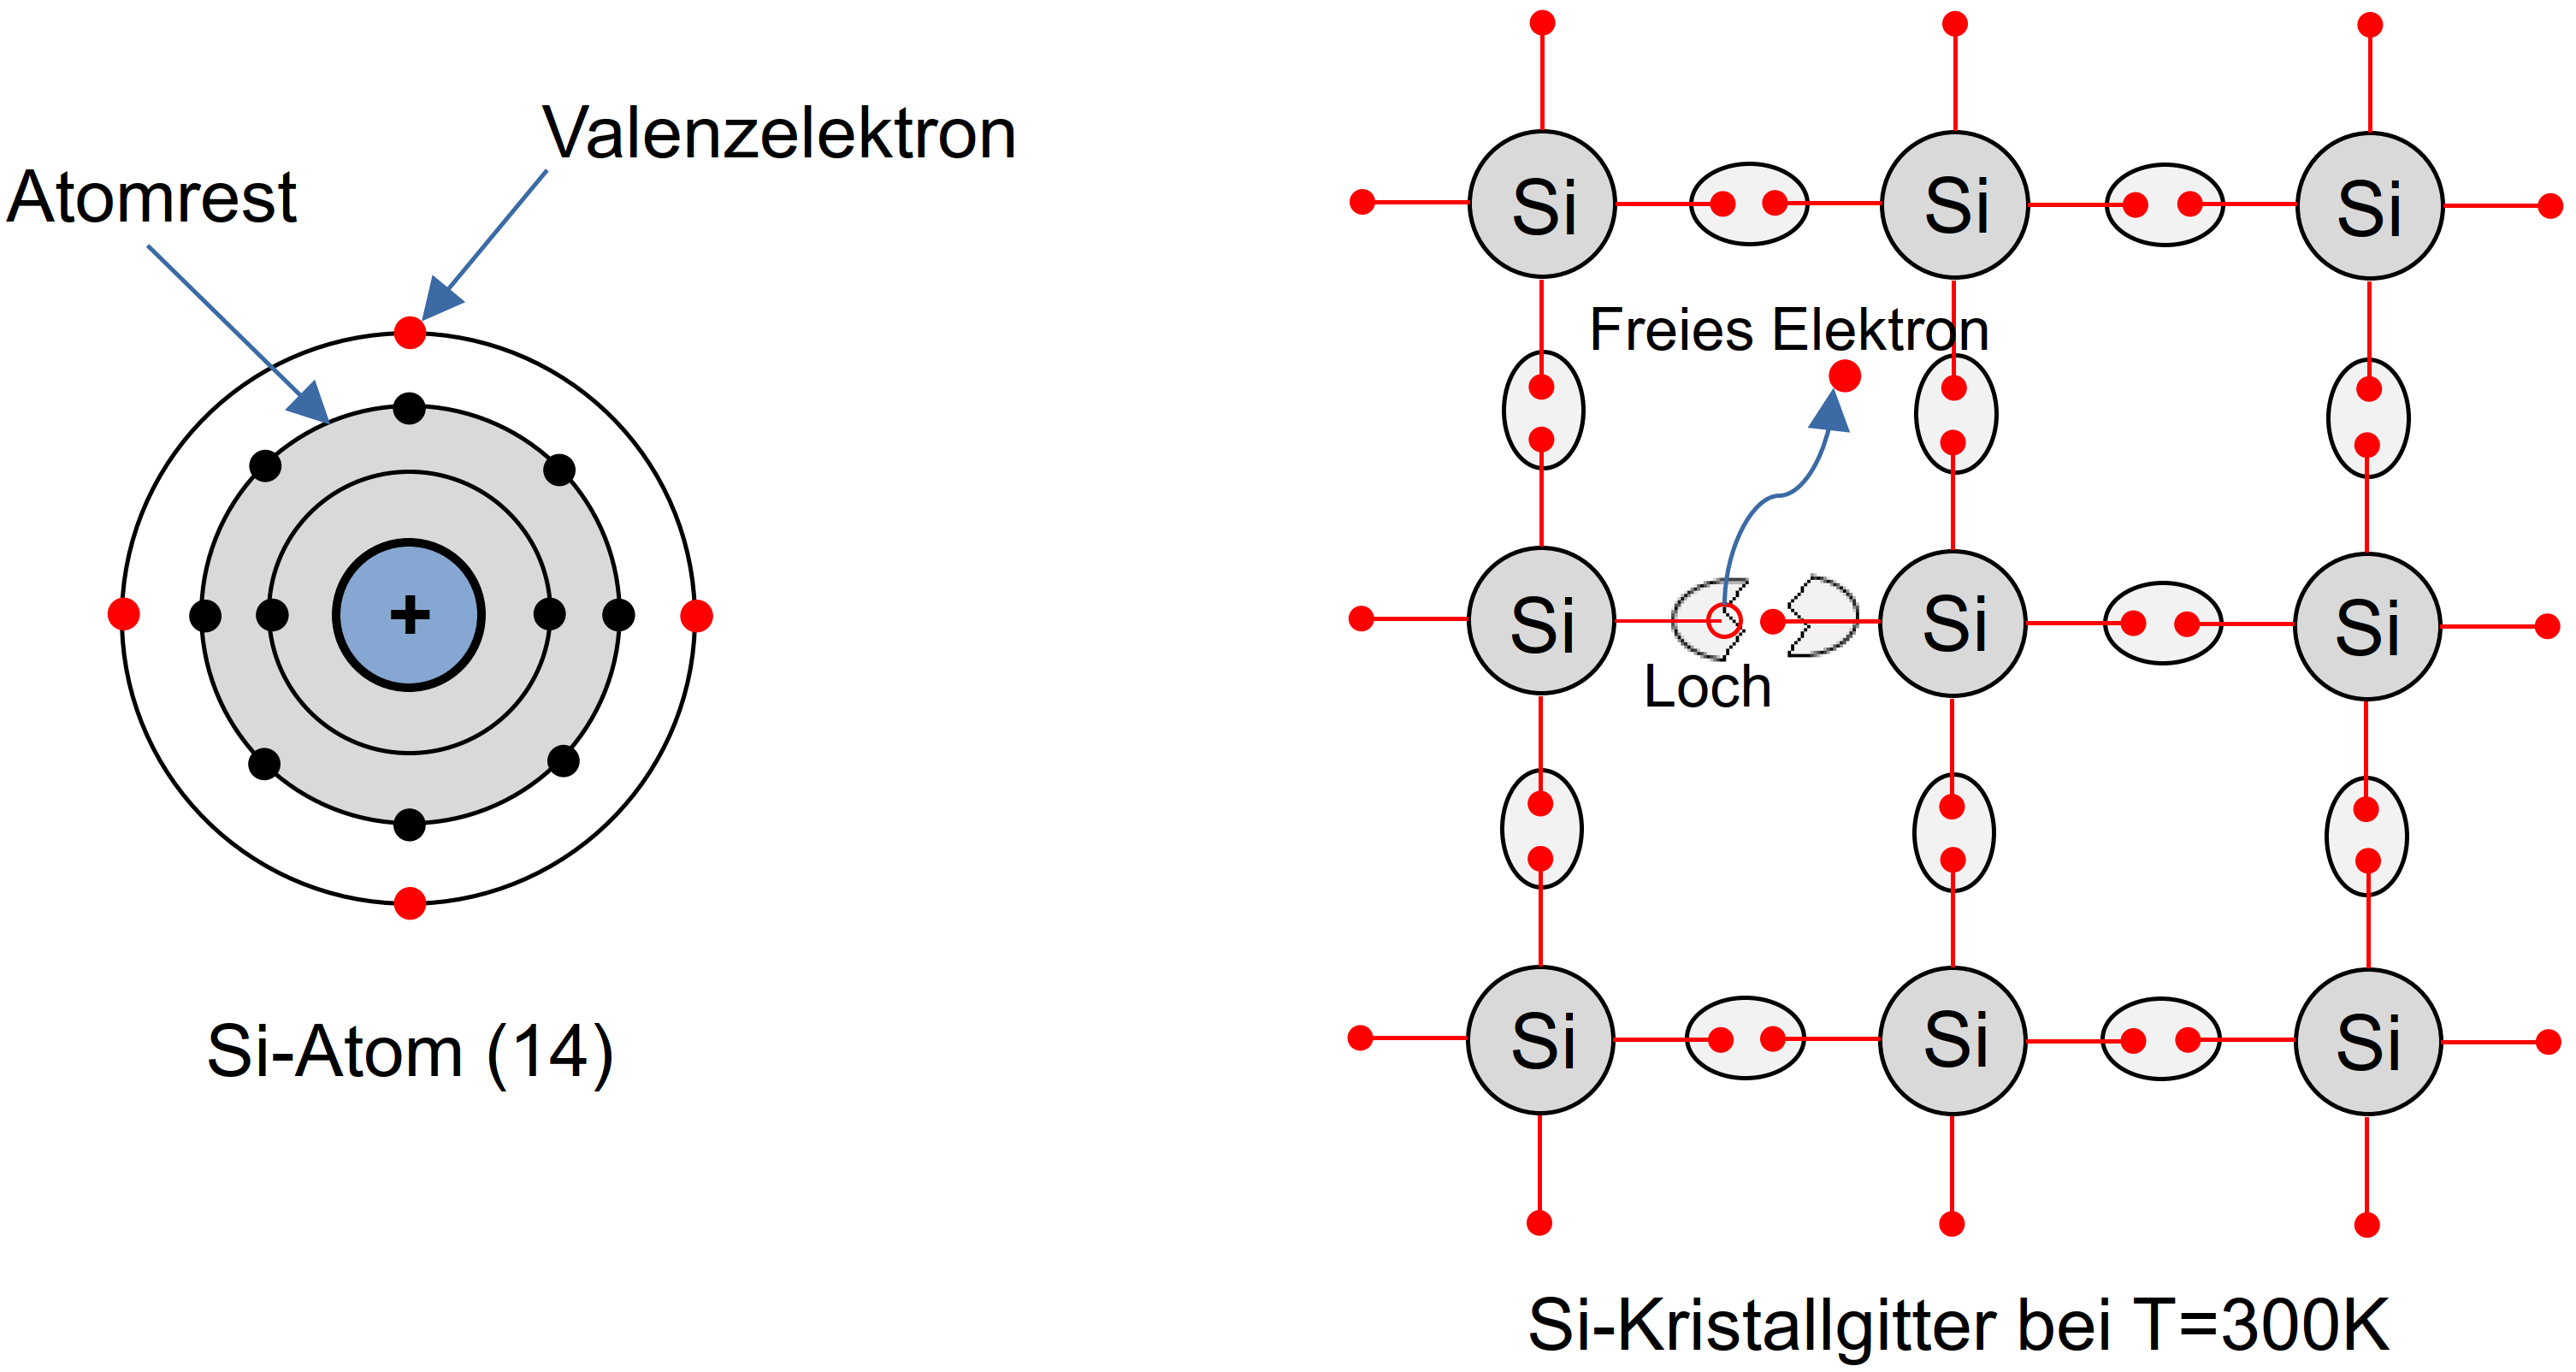
\includegraphics[width=\columnwidth]{images/Bild3.png}

\subsubsection{Störstellenleitung}
Durch eine Dotierung des Halbleitermaterials mit Fremdatomen ist es möglich 
die Ladungsträgerdichte effizient zu kontrollieren.\\
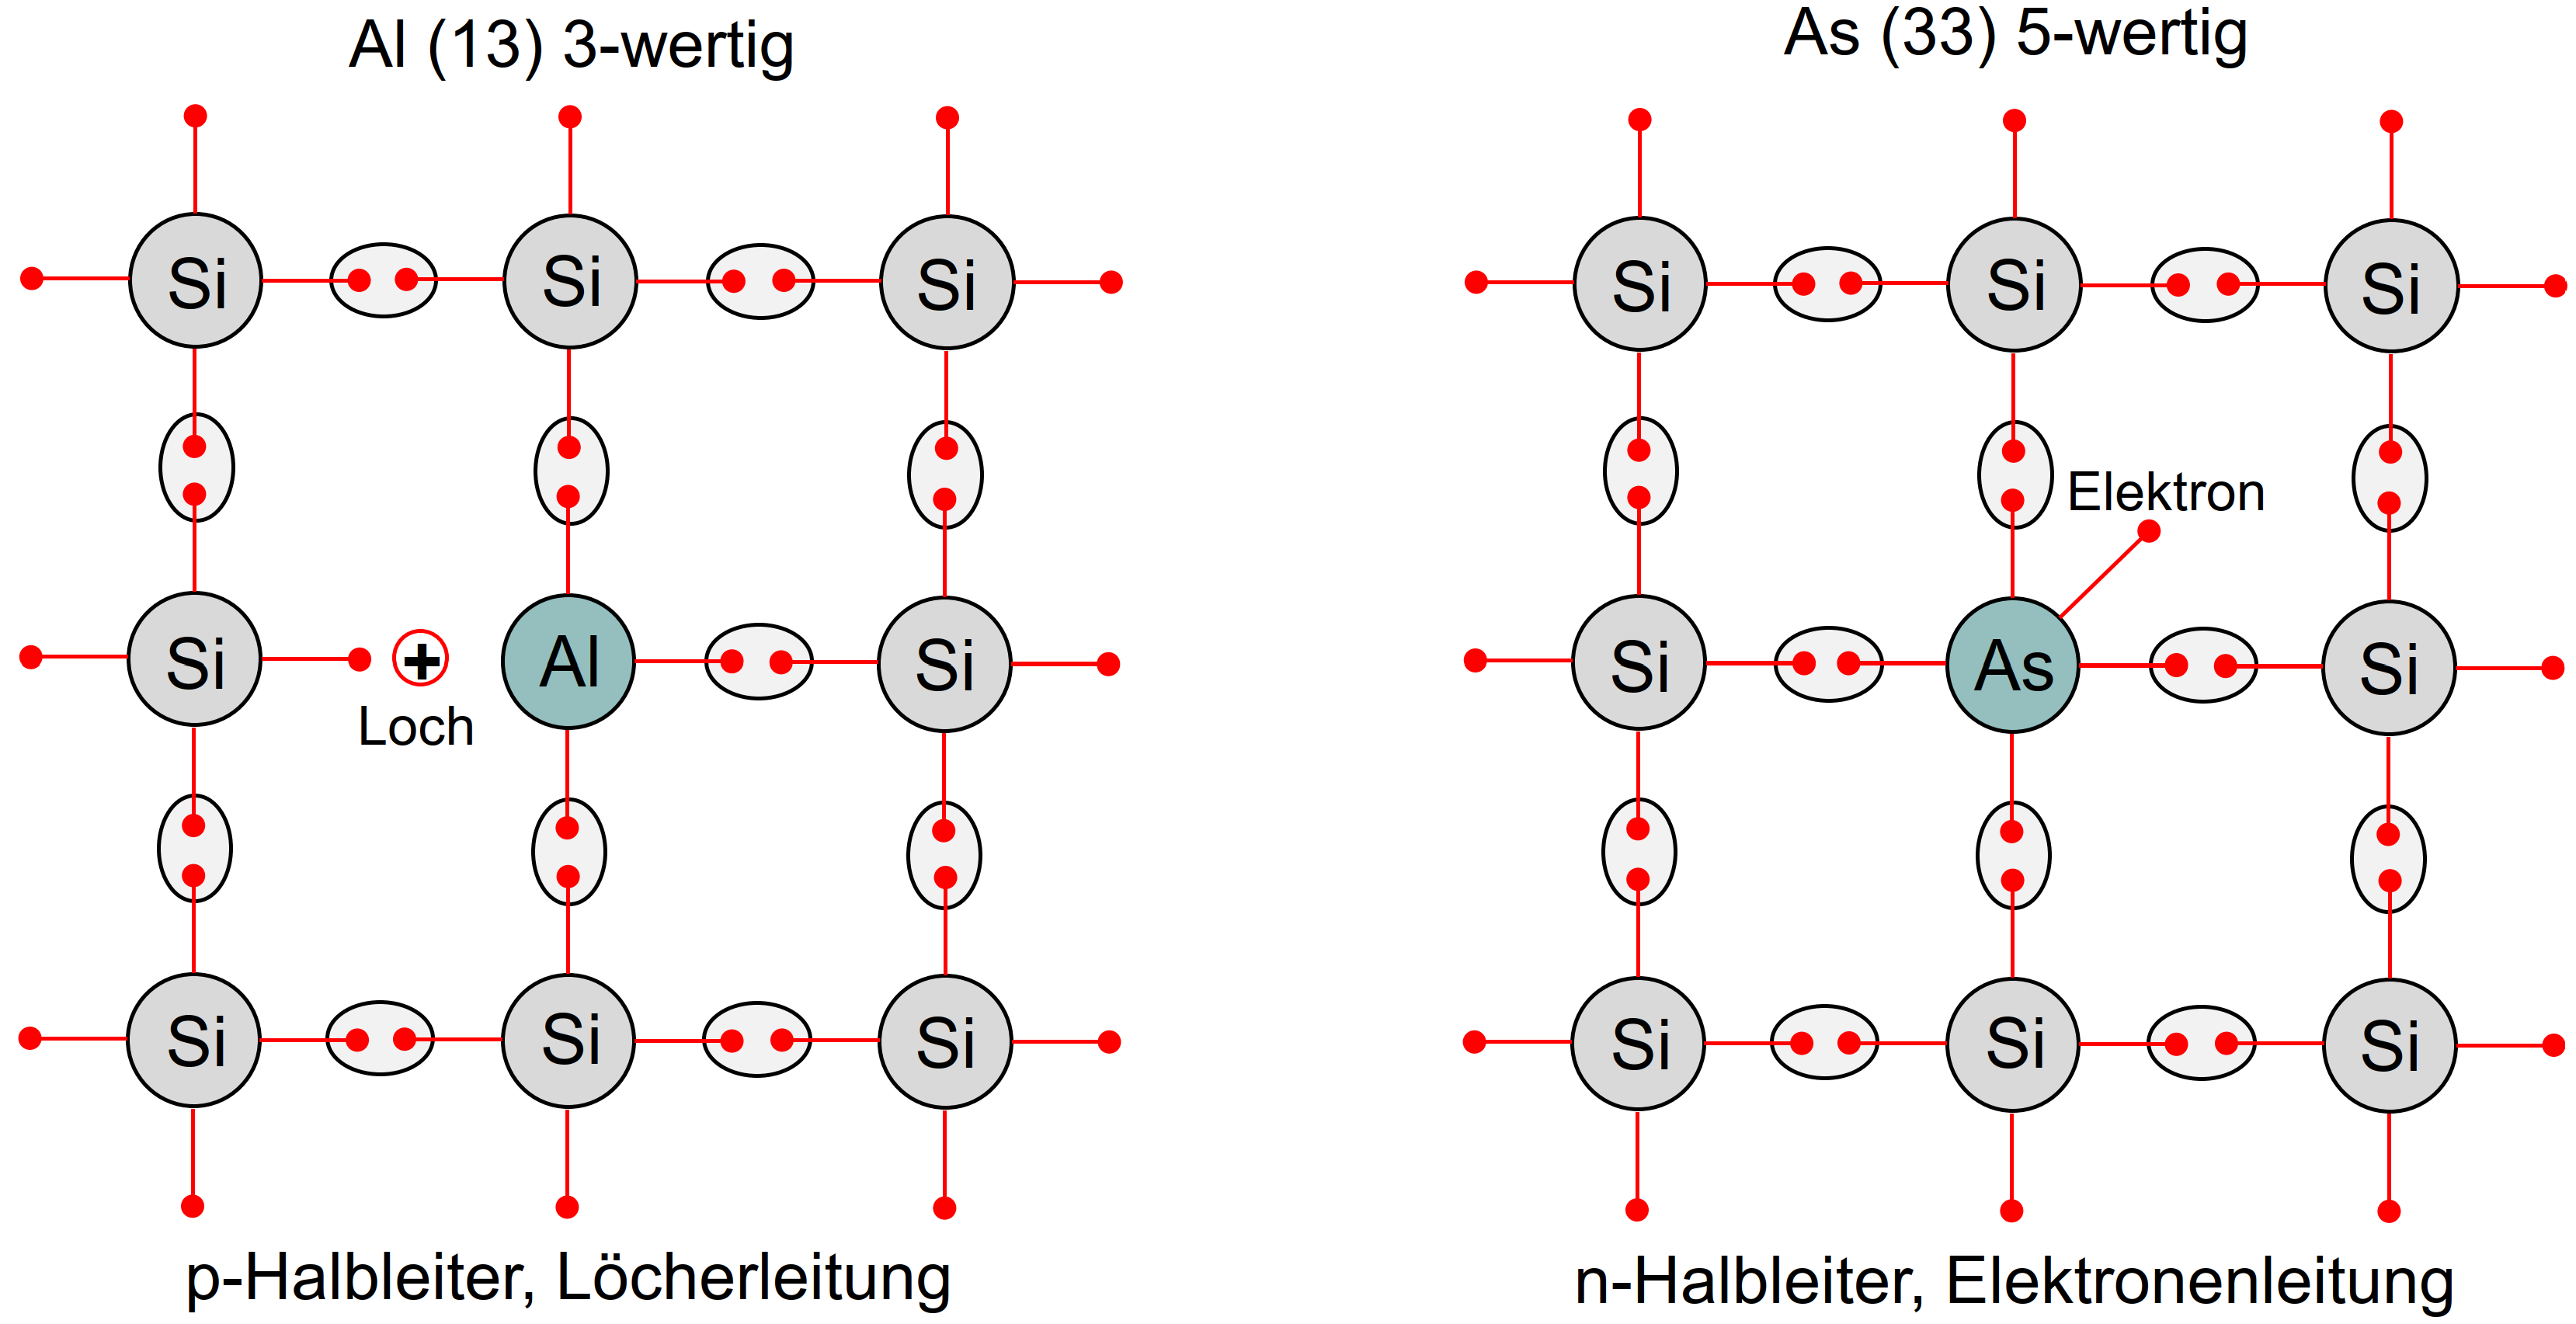
\includegraphics[width=\columnwidth]{images/Bild4.png}

\subsubsection{pn-Übergang}
\begin{minipage}[c]{0.48\columnwidth}
    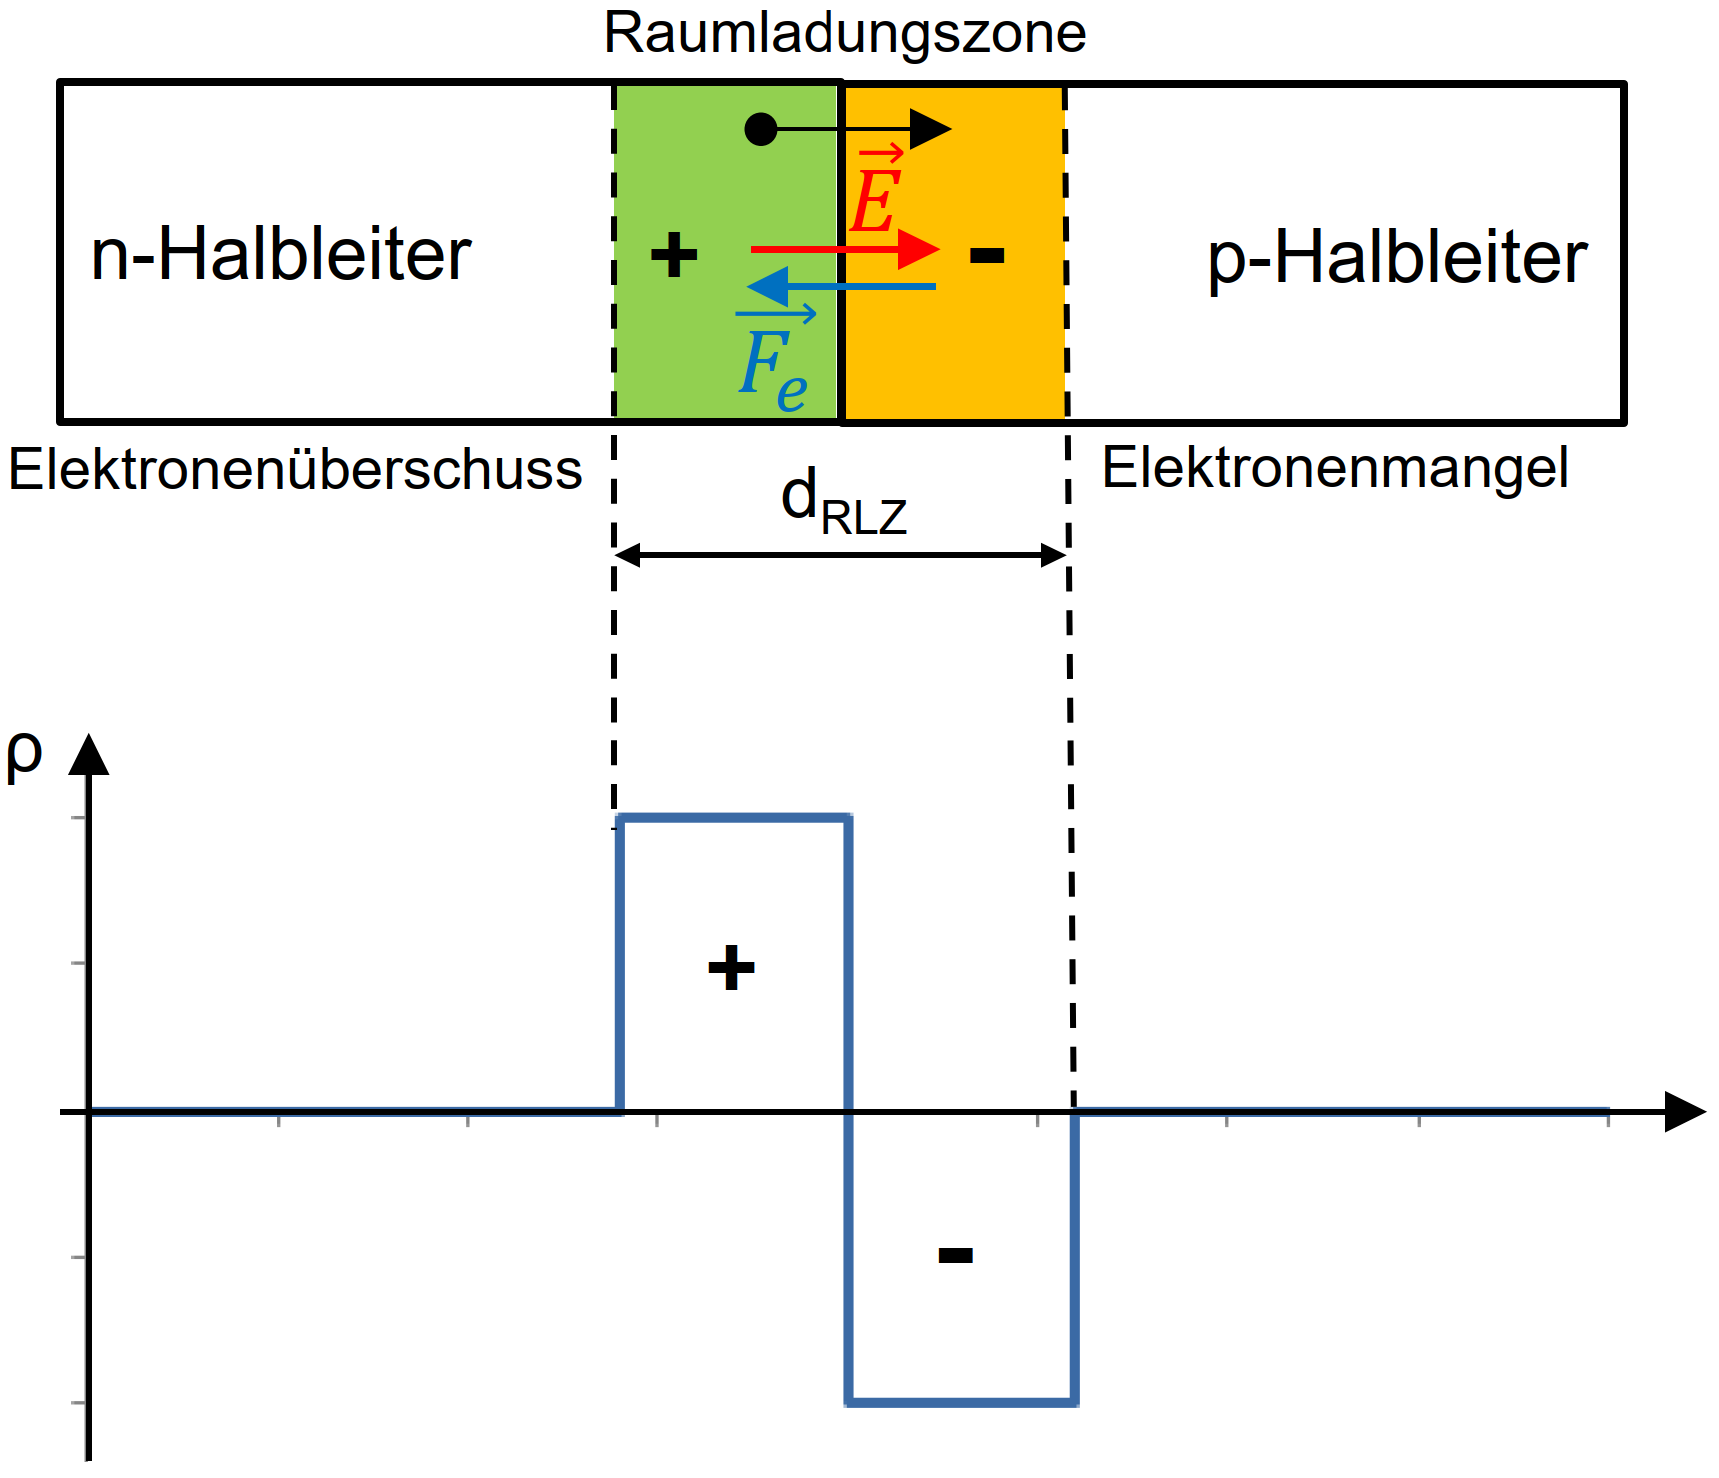
\includegraphics[width=\columnwidth]{images/Bild5.png}\\
\end{minipage}
\hfill
\begin{minipage}[c]{0.48\columnwidth}
    \textbf{Der Diffusionsstrom} wird durch den Ladungsträgeraustausch zwischen beiden Halbleitergebieten erzeugt und dadurch verschwinden in der Grenzschicht alle freien Ladungsträger.\\\\
    Durch die Elektronenabwanderung entsteht im n-Teil des Grenzgebiets die ortsfeste positive Ladung (+). Die eindiffundierten Elektronen erzeugen im p-Teil des Grenzgebiets die ortsfeste negative Ladung (-). Die ortsfesten Ladungen erzeugen das elektrische Feld (E) in der Raumladungszone und damit auch \textbf{den Driftstrom}.\\
\end{minipage}
Der Driftstrom ist gegen den Diffusionsstrom gerichtet. So bald die Ströme gleich sind, ist eine stabile Raumladungszone etabliert.

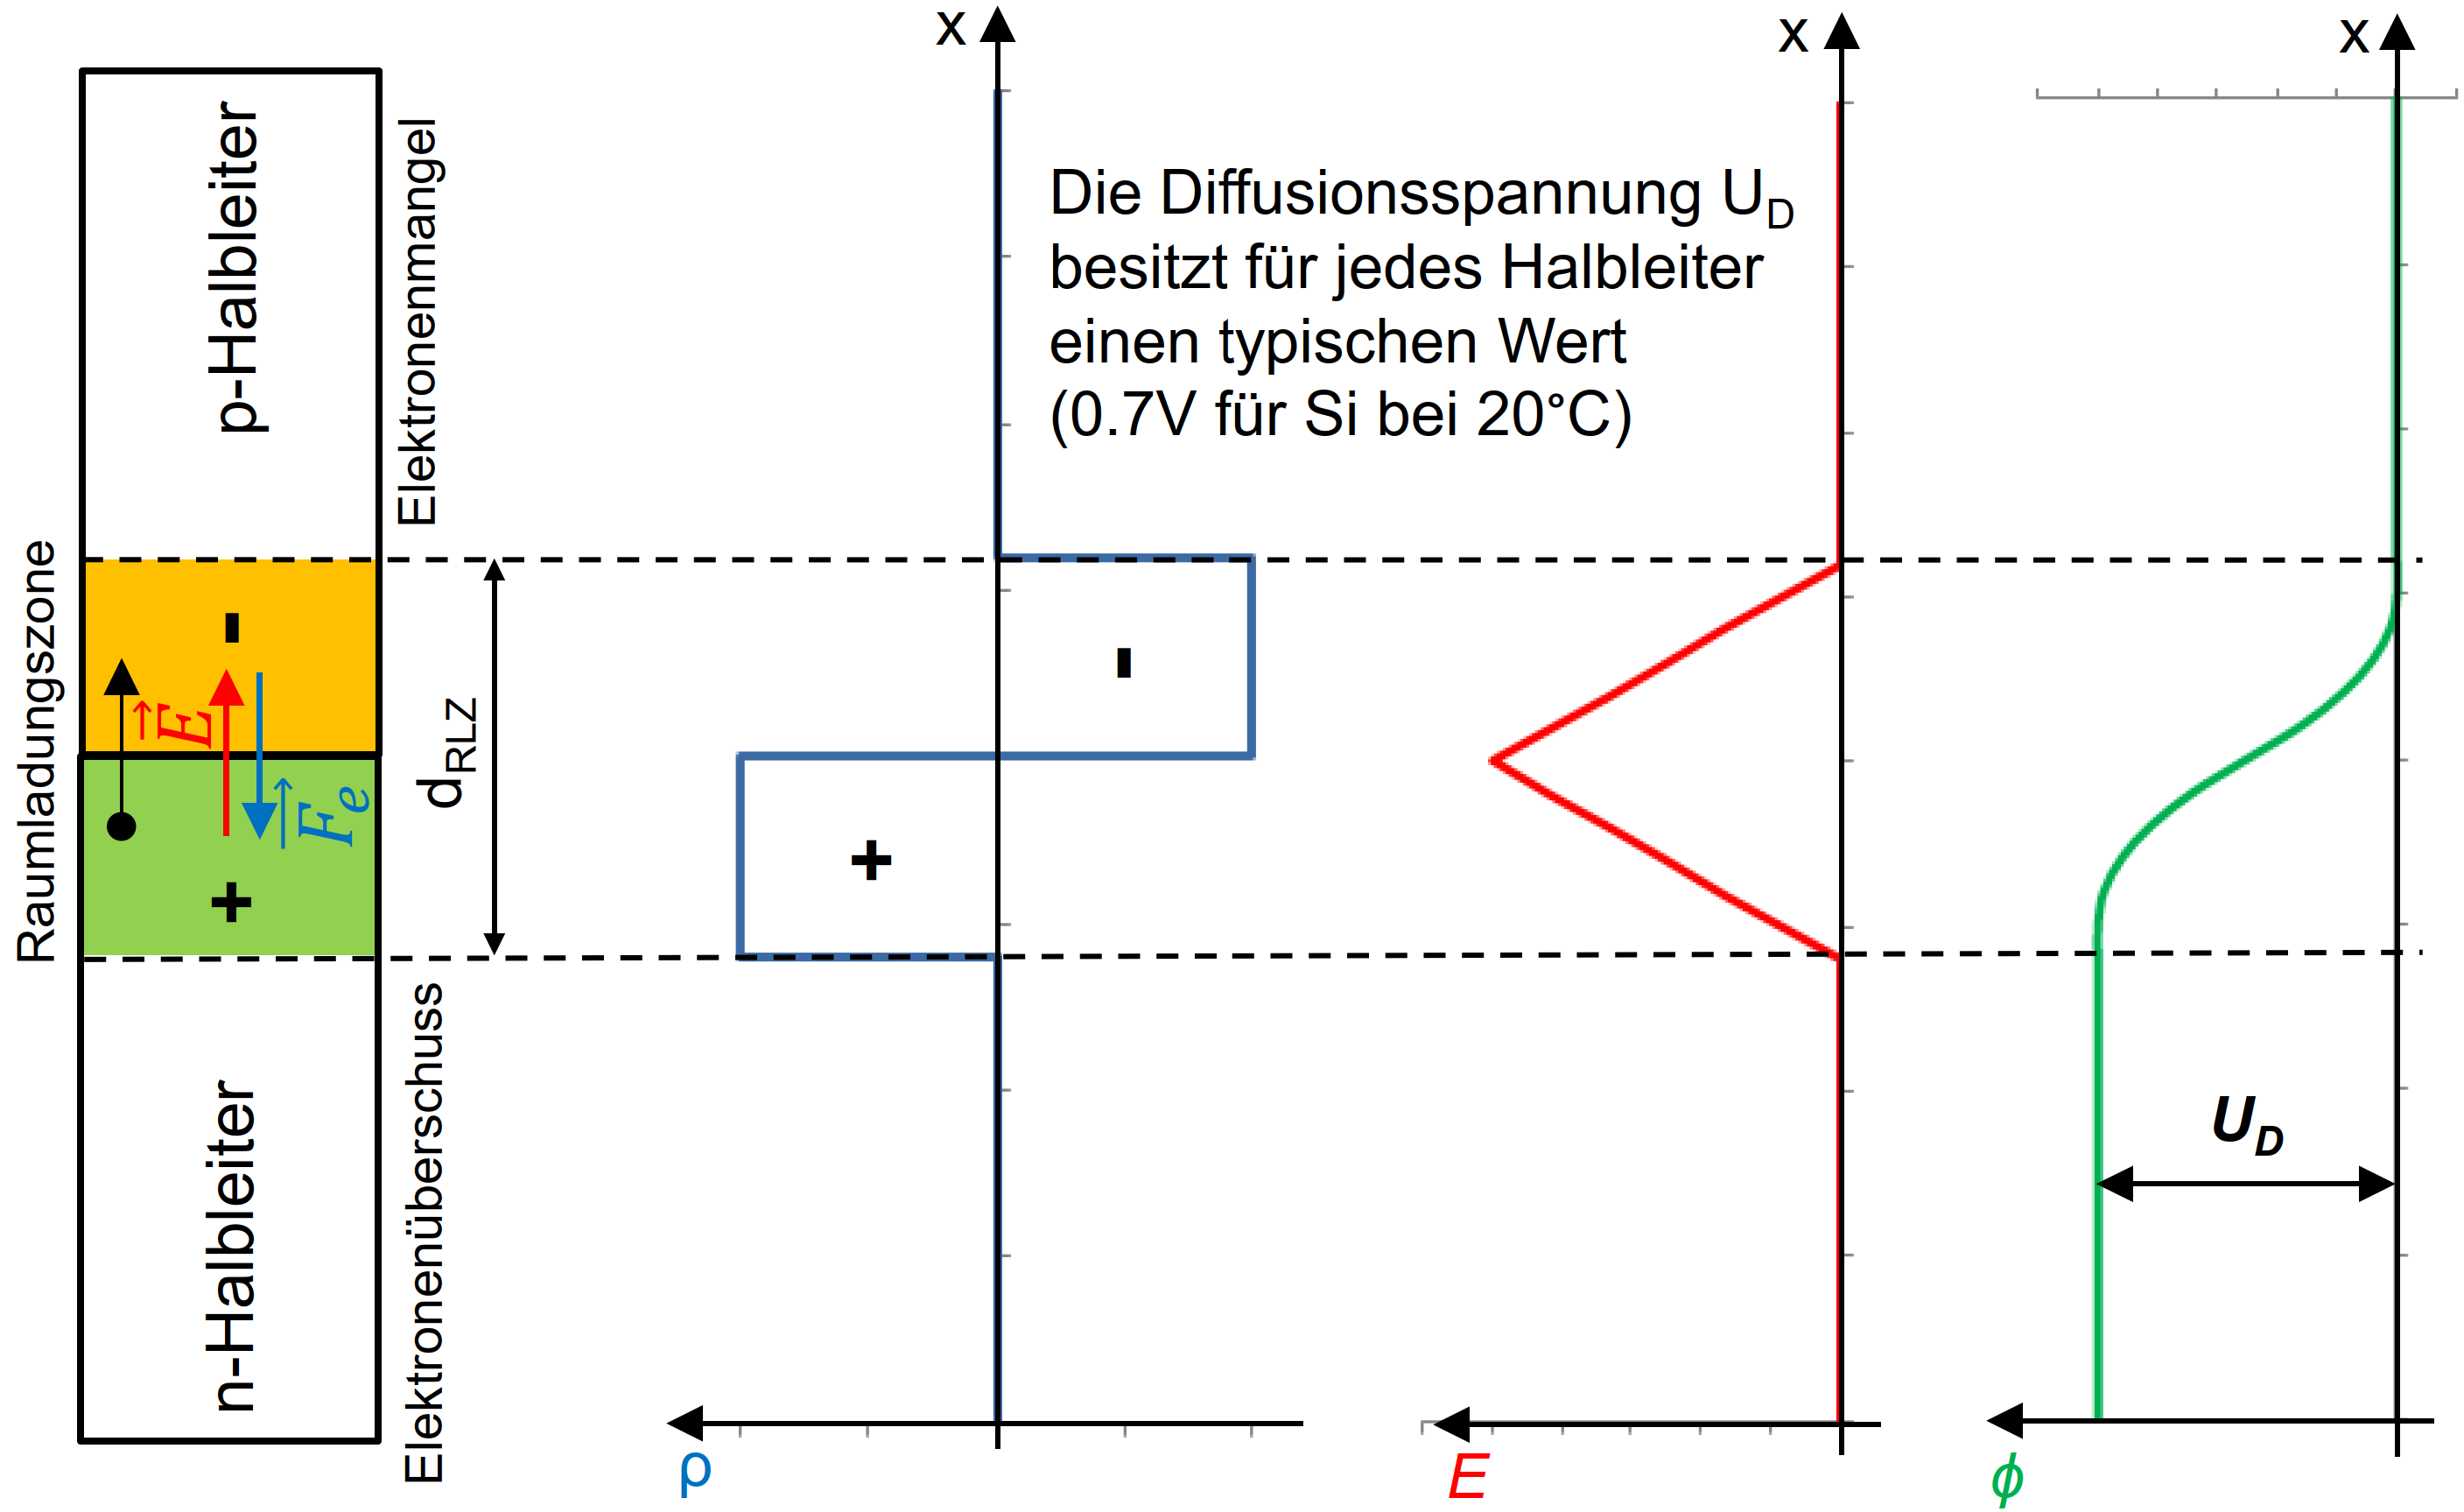
\includegraphics[width=\columnwidth]{images/Bild6.png}\\
